%%%%%%%%%%%%%%%%%%%%%%%%%%%%%%%%%%%%%%%%%%%%%%%%%%%%%%%%%%%%%%%%%%%%%
% PREAMBLE
%%%%%%%%%%%%%%%%%%%%%%%%%%%%%%%%%%%%%%%%%%%%%%%%%%%%%%%%%%%%%%%%%%%%%
%
% The following two commands will generate a PDF that follows all the 
% requirements for submission and peer review.  Uncomment these commands to 
% generate this output (and comment out the two lines below.)
%
% DOUBLE SPACE VERSION FOR SUBMISSION TO THE AMS
\documentclass[12pt]{article}
\usepackage{ametsoc}
%
% The following two commands will generate a single space, double column paper 
% that closely matches an AMS journal page.  Uncomment these commands to 
% generate this output (and comment out the two lines above. FOR AUTHOR USE 
% ONLY. PAPERS SUBMITTED IN THIS FORMAT WILL BE RETURNED TO THE AUTHOR for 
% submission with the correct formatting.
%
% TWO COLUMN JOURNAL PAGE LAYOUT FOR AUTHOR USE ONLY
%%%%\documentclass[10pt]{article}
%%%%\usepackage{ametsoc2col}
%
%%%%%%%%%%%%%%%%%%%%%%%%%%%%%%%%%%%%%%%%%%%%%%%%%%%%%%%%%%%%%%%%%%%%%
% ABSTRACT
%
% Enter your Abstract here
%%%%%%%%%%%%%%%%%%%%%%%%%%%%%%%%%%%%%%%%%%%%%%%%%%%%%%%%%%%%%%%%%%%%%
\newcommand{\myabstract}{
Direct calculations of the entrainment and detrainment of air into and out of
clouds require a knowledge of the relative velocity difference between the air 
and the cloud surface.  However, the discrete numerical model grids force the 
distance moved by a cloud surface over a time step to be either zero or the 
width of a model grid cell.  Here we present a method for the subgrid 
interpolation of a cloud surface on a discrete numerical model grid.  This
method is used to calculate entrainment and detrainment rates for an LES model,
which are compared with rates inferred from bulk conserved tracer
calculations.  Our method results in entrainment and detrainment values that
are 1.5 to 3 times as large as values calculated via bulk tracers.  Correcting 
the entrainment and detrainment values to account for the effect of the moist 
cloud shell corrects this over-estimate.  The correlation of values calculated 
via the two methods is nearly unity, suggesting our method captures the 
dynamics of entrainment and detrainment well.
}
%
\begin{document}
%
%%%%%%%%%%%%%%%%%%%%%%%%%%%%%%%%%%%%%%%%%%%%%%%%%%%%%%%%%%%%%%%%%%%%%
% TITLE
%
% Enter your TITLE here
%%%%%%%%%%%%%%%%%%%%%%%%%%%%%%%%%%%%%%%%%%%%%%%%%%%%%%%%%%%%%%%%%%%%%
\title{\textbf{\large{Interpolation of LES cloud surfaces for use in direct
calculations of entrainment and detrainment}}}
%
% Author names, with corresponding author information. 
% [Update and move the \thanks{...} block as appropriate.]
%
\author{\textsc{Jordan T. Dawe}
	\thanks{\textit{Corresponding author address:} 
	Jordan T. Dawe, 
        Department of Earth and Ocean Sciences, 
        University of British Columbia, 
	6339 Stores Road, 
        Vancouver, BC, 
        V6T 1Z4. 
	\newline{E-mail: jdawe@eos.ubc.ca}}\quad\textsc{and Phillip Austin}\\
\textit{\footnotesize{Department of Earth and Ocean Sciences, 
                      University of British Columbia, Vancouver, BC}}
}
%
% Formatting done here...Authors should skip over this.  See above for abstract.
\ifthenelse{\boolean{dc}}
{
\twocolumn[
\begin{@twocolumnfalse}
\amstitle

% Start Abstract (Enter your Abstract above.  Do not enter any text here)
\begin{center}
\begin{minipage}{13.0cm}
\begin{abstract}
	\myabstract
	\newline
	\begin{center}
		\rule{38mm}{0.2mm}
	\end{center}
\end{abstract}
\end{minipage}
\end{center}
\end{@twocolumnfalse}
]
}
{
\amstitle
\begin{abstract}
\myabstract
\end{abstract}
}
%%%%%%%%%%%%%%%%%%%%%%%%%%%%%%%%%%%%%%%%%%%%%%%%%%%%%%%%%%%%%%%%%%%%%
% MAIN BODY OF PAPER
%%%%%%%%%%%%%%%%%%%%%%%%%%%%%%%%%%%%%%%%%%%%%%%%%%%%%%%%%%%%%%%%%%%%%

\section{Introduction}

The largest uncertainties in climate sensitivity estimates from Global
Circulation Model (GCM) simulations come from the subgridscale
parameterization of low clouds \citep{Colman2003,Bony2005,Webb2006}.
Specifically, stratocumulus clouds and the transition regime from
stratocumulus to trade cumulus are the dominant source of variance
between models in the estimation of the cloud radiative response to
changing climate \citep{Williams2009}.

Proper simulation of the subgridscale effect of cumulus clouds in
GCMs requires understanding the rates at which air is entrained into
and detrained from the clouds. Cloud entrainment and detrainment rates
exert influences on profiles of cloud properties, the height of the
cloud tops, the amount of heat and moisture the clouds transport upwards,
and the heights at which the clouds deposit that heat and moisture.
They also have effects on the vertical transport of aerosols out of
the boundary layer and the rate at which chemical reactions can occur
in those aerosols \citep{Barahona2007,Anldrejczuk2008}. 
Several approaches to the parametrization of entrainment
and detrainment rates have been proposed, including 
\citep{Lock2000,Bretherton2009,Siebesma2007}.  *PA -- words here*


Large Eddy Simulation (LES) is an important tool used in the study
of cloud entrainment and detrainment. LES models achieve grid resolutions
on the order of 10-100 m, well within the domain of the Kolmagorov -5/3
turbulence spectrum. This allows for a relatively simple turbulence
model that captures the important statistics of the subgridscale eddy
fluxes and thus, an accurate representation of the atmospheric physics
of a domain $\approx$ 10 km$^{2}$, which is enough to simulate a field of shallow clouds. 
LES simulations can be ground-truthed against results taken from field surveys 
such as the Barbados Oceanographic and Meteorological
Experiment \citep[BOMEX;][]{Holland1973} or the Atmospheric Radiation 
Measurement \citep[ARM;][]{Brown2002} Program, and such comparisons 
show good agreement between LES and data.

Several recent studies have looked at the life cycle of individual
clouds taken from LES models, trying to break the cloud field into
its component parts. Estimates of entrainment and detrainment rates
for individual clouds would be quite useful in these types of studies,
but are difficult to achieve. Entrainment and detrainment rates are 
typically calculated in LES simulations by recording budgets
of bulk conserved tracer variables, such as the total humidity or
the liquid water moist static energy, and inferring the amount of
fluid exchange between cloud and clear air that is needed to explain
the rate at which that tracer is being vertically advected within
the cloud field. These budgets typically assume the clouds and the
cloud environment are horizontally homogeneous slabs; this is a much
less accurate assumption on the level of an individual cloud.

Alternatively, entrainment and detrainment could simply be calculated
directly from the LES velocity and humidity field.  \cite{Siebesma1998} 
defines Entrainment and Detrainment as

\begin{equation}
E = -\frac{1}{A}\oint_{\mathbf{\hat{n}}\cdot(\mathbf{u} - \mathbf{u_i}) < 0}
\mathbf{\hat{n}}\cdot(\mathbf{u}-\mathbf{u_i})dl
\end{equation}
\begin{equation}
D = \frac{1}{A}\oint_{\mathbf{\hat{n}}\cdot(\mathbf{u} - \mathbf{u_i}) > 0}
\mathbf{\hat{n}}\cdot(\mathbf{u}-\mathbf{u_i})dl
\end{equation}

where $E$ and $D$ are the entrainment and detrainment rates in kg 
m$^{-3}$ s$^{-1}$, $u$ is the velocity of the air in m s$^{-1}$, $u_i$ is the 
velocity of the cloud surface in m s$^{-1}$, A is the area of the cloud in m,
$\mathbf{\hat{n}}$ is a unit vector directed out the cloud surface, and the 
path integral is taken around the cloud surface at a constant vertical level.
However, the accuracy of this method suffers from the need to calculate the 
velocity of the air relative to the cloud surface.  In reality these velocities 
are very nearly identical, \textasciitilde{} 1-2 m s$^{-1}$, but the discrete 
nature of the LES model grid forces the modelled surface velocity to be either 
0 m s$^{-1}$ or $\Delta x / \Delta t \approx$ 15-30 m s$^{-1}$, where 
$\Delta x$ is the model grid spacing and $\Delta t$ is the model time step.  The
surface of the cloud only moves when a grid cell's humidity reaches saturation, 
and when it does, an entire grid cell worth of fluid leaves or enters the cloud.
This causes both the entrainment and detrainment to be over-estimated.

Here we present a method for calculation of the cloud entrainment and 
detrainment rates that relies on interpolation of the subgrid location 
of the cloud surface.  We believe this method can be used to produce accurate
estimates of the cloud entrainment and detrainment rates for individual LES
clouds.  In section 2 we describe this method, in section 3 we describe the 
model configuration we used to test this method, in section 4 we compare this
calculation with entrainment and detrainment rates calculated using bulk
conserved tracer budgets, in section 5 we discuss our results, and in section 6
we present our conclusions.  

%==============================================================================

\section{Method}

Consider a 3-d numerical model grid cell containing a cloud surface with 
normal vector $\mathbf{C}$, where $\mathbf{C}$ points outward from the cloud.
This surface, combined with $\mathbf{W}$, the portion of the grid cell walls
that lie within the cloud, encloses a cloud volume $V$ with surface $\mathbf{A}
= \mathbf{C} \cup \mathbf{W}$.  \cite{Siebesma1998} gives the net entrainment and
detrainment over the cloud surface to be:
\begin{equation}
\label{eq:E_minus_D} 
E - D = \int_C \rho ( \mathbf{u} -  \mathbf{u_i}) \cdot d\mathbf{C},
\end{equation}
where $\rho$ is the air density in kg m$^{-3}$, $\mathbf{u}$ is the velocity
of the air in m s$^{-1}$ and $\mathbf{u_i}$ is the velocity of the cloud 
interface.  Calculating this integral requires knowledge of the velocity field
over the surface of $\mathbf{C}$ and the time evolution of $\mathbf{C}$, 
neither of which is easily calculated in a numerical model.  Instead, we seek a
simplified but equivalent calculation.

To calculate the velocity of the cloud interface, we make use of the Leibnitz 
Theorem:
\begin{equation}
\label{eq:leibnitz} 
\frac{d}{dt}\int_{V(t)} \rho dV = 
  \int_{V(t)} \frac{\partial \rho}{ \partial t} dV 
  + \int_{A(t)} \rho \mathbf{u_i}\cdot d\mathbf{A}.
\end{equation}
Since the walls of the grid cell do not move, $\mathbf{u_i}$ is 0 over 
$\mathbf{W}$.  If we also assume ${\partial \rho}/{ \partial t} \approx 0$, we
get
\begin{equation}
\label{eq:leibnitz2} 
    \rho \frac{d}{dt}\int_{V(t)} dV = 
    \int_{C(t)} \rho \mathbf{u_i}\cdot d\mathbf{C}.
\end{equation}
We then combine equations (\ref{eq:E_minus_D}) and (\ref{eq:leibnitz2}) to give:
\begin{equation}
\label{eq:step1} 
      E - D = \int_C \rho \mathbf{u} \cdot d\mathbf{C} 
            - \rho \frac{d}{dt}\int_{V(t)} dV.
\end{equation}

Next we apply the divergence theorem to simplify the flux integral through 
$\mathbf{C}$:
\begin{equation}
\label{eq:divergence} 
\int_{V} \nabla \cdot (\rho \mathbf{u}) dV = 
  \int_{A} \rho \mathbf{u}\cdot d\mathbf{A}
\end{equation}
Due to mass conservation, $\nabla \cdot (\rho \mathbf{u}) = 0$, which implies
\begin{equation}
\label{eq:divergence3} 
\int_{C} \rho \mathbf{u}\cdot d\mathbf{C} = - \int_{W} \rho \mathbf{u}\cdot d\mathbf{W}
\end{equation}
since $\mathbf{A}$ is the union of $\mathbf{C}$ and $\mathbf{W}$.  Substituting
this into (\ref{eq:step1}) results in
\begin{equation}
\label{eq:entrainment_detrainment} 
E - D = - \int_W \rho \mathbf{u} \cdot d\mathbf{W} - \rho \frac{dV}{dt}.
\end{equation}
Therefore, we can find the entrainment and detrainment by calculating the mass
flux through the cloudy portion of the grid cell walls and the rate of change
of the cloud volume inside the grid cell.  If equation $E - D$ is greater than 
zero, the total is applied to entrainment and if less than zero, to 
detrainment.  This technique works equally well for flux through any surface 
that can be defined within the model; in this paper we perform these 
calculations for the cloud core, which we define following \cite{Siebesma1995} 
as fluid having condensed liquid water, upward velocity, and positive buoyancy 
relative to the horizontal mean.  

Calculating the mass flux through the grid cell walls can be accomplished using 
the numerical model's advection routine; this is trivial for a model using an 
Arakawa C-grid, while interpolation can give fluxes for other grid 
configurations.  We assume the mass flux is constant over the grid cell wall.  
To calculate the portion of the grid cell walls within the cloud and the cloud 
volume inside the grid cell we interpolate the location of the cloud surface at 
each time step.  Next, we describe the interpolation schemes we use for this 
purpose.

%-----------------------------------------------------------------------------

\subsection{Cloud Surface Interpolation}

There are a multitude of interpolation schemes that can be used to determine 
the cloud volume and cloudy cell wall area in a numerical model.  The simplest 
would be to assume that saturated grid cells are completely filled with cloud 
and unsaturated grid cells have no cloud at all.  We refer to this as the "no 
interpolation" case.  Since the cloud surface only moves when a whole grid cell 
undergoes condensation or evaporation, this will result in poor estimates of 
$dV/dt$ and $\mathbf{S}$, which will then overestimate the entrainment and 
detrainment.

At the other end of the range of interpolation schemes, we can use linear (or 
higher order) interpolation to estimate the surface where the total water 
equals the saturated humidity and calculate the cloud volume and cell surface 
areas at each time step.  Several standard techniques exist for this kind of 
calculation in the field of computer visualization, such as the Marching 
Cubes algorithm \citep{Lorensen1987}.  Instead we have implemented two related 
schemes that rely on subdividing the grid cells into regular sub-cells, finding 
the location of the cloud surface within these sub-cells, and then reassembling 
the cells to construct the location of the cloud surface.  The first scheme 
gives a coarse approximation to the cloud surface, but requires a relatively 
small amount of computation.  The second scheme requires more computation, but 
produces a more accurate cloud surface.

%------------

\subsubsection{Pyramidal Interpolation}

The first of these methods, which we refer to as the "pyramidal interpolation" 
case, involves splitting the cell into six pyramids  
(Figure \ref{fig:pyramid_scheme}).  Next, we compute the value of 
$q_{diff} = q_t - q_{sat}(T, p)$, where $q_t$ is the total specific water and
$q_{sat}(T, p)$ is the saturated specific humidity, all in kg kg$^{-1}$.  
$q_{diff}$ is positive for cloudy points, negative for clear points, and zero 
at the cloud surface, representing the moisture excess or deficiency relative 
to the cloud surface.  Then we linearly interpolate these values to the walls 
of the nearest neighbour cells in all six directions.  Thus, for each of the 
six pyramids we have the grid cell value of $q_{diff}$ at the pyramid apex, and
an interpolated value at the center of the pyramid base. If both values are 
less than zero, the pyramid contains no cloud; if both are greater than zero, 
the pyramid is filled with cloud; otherwise, the fractional distance between 
the pyramid apex and base at which $q_{diff} = 0$ is calculated via linear 
interpolation:
\begin{equation}
\label{eq:q_diff_interpolation}
x = \frac{q_{diff}(x_1)}{q_{diff}(x_2) - q_{diff}(x_1)}.
\end{equation}
The volume of the cloudy portion of the pyramid, expressed as a fraction of the 
grid cell volume, is calculated as:
\begin{equation}
V = \frac{1}{6}x^3.
\end{equation}
This calculation is then repeated for $\Delta\theta_v = \theta_v - 
\overline{\theta_v}$, where $\theta_v$ is the virtual potential temperature in 
Kelvins and $\overline{\theta_v}$ is the horizontal mean of the virtual 
potential temperature.  The $x$ value that returns the smaller cloud volume is 
taken to be the location of the cloud core surface, cutting the pyramid 
parallel to the pyramid base.  Finally, the fractional cloud area at the wall 
of the cell is simply set to either one or zero, depending on the values of 
$q_{diff}$ and $\theta_v$ at the pyramid base.

%------------

\subsubsection{Tetrahedradal Interpolation}

The second interpolation method, which we refer to as the "tetrahedral 
interpolation" case, involves splitting the cube into six pyramids, then 
splitting each pyramid into eight tetrahedrons. This results in forty-eight 
tetrahedrons in total, each composed of four vertices located at the grid cell 
centre, the centre of a grid cell wall, the centre of a grid cell edge, and 
a grid cell corner.  The values of $q_{diff}$ and $\theta_v$ are linearly 
interpolated to each of these points, then used to find the location of the 
cloud surface.  This method is more accurate than the pyramidal interpolation 
scheme, but with much higher computational requirements.

The surface is defined in a similar way to the Marching Cubes algorithm 
\citep{Lorensen1987}.  As each tetrahedron has four vertexes, each of which can
either be cloudy or clear, there are 16 possible cases that must be considered. 
Many of these cases share symmetries, reducing the number of independent cases 
to four classes.  If the vertexes of a tetrahedron are all cloudy or all clear, 
the cloud surface does not pass through the tetrahedron.  If only one of the 
vertexes is clear (or conversely, only one is cloudy) than that corner of the 
tetrahedron is cut by a triangle that intersects the tetrahedron edges where 
$q_{diff}=0$ (or $\theta_v = 0$, depending on which results in a smaller cloud 
volume), determined by linearly interpolating the values at the vertexes; this 
accounts for eight of the cases.  The remaining six cases have two cloudy 
vertexes two clear vertexes, and result in the tetrahedron being cut by two 
triangles which share a common edge.

Once the geometry of the case is determined, the area of the cloudy portion of
the model grid cell wall is calculated by dividing the cloudy area into 
triangles and summing the triangle areas
\begin{equation}
A = \frac{|(\mathbf{b - c}) \times (\mathbf{a - c})|}{2},
\end{equation}
where $\mathbf{a}$, $\mathbf{b}$, $\mathbf{c}$ are the position vectors of the 
vertices of the triangles.  Similarly, the volume of the cut tetrahedron is 
calculated by subdividing it into smaller tetrahedrons, and summing the volumes 
of the sub-tetrahedrons using
\begin{equation}
V = \frac{|\mathbf{a - d} \cdot ((\mathbf{b - d}) \times (\mathbf{c - d}))|}{6},
\end{equation}
where $\mathbf{a}$, $\mathbf{b}$, $\mathbf{c}$, and $\mathbf{d}$ are the 
position vectors of the vertices of the sub-tetrahedrons.

%==============================================================================

\section{Model Description}

We have implemented these surface interpolation schemes in the System for 
Atmospheric Modelling \citep[SAM;][]{Khairoutdinov2003}, allowing the model to 
calculate cloud core entrainment and detrainment at every time step.  We have 
run these schemes in a standard GCSS Barbados Oceanographic and Meteorological 
Experiment (BOMEX) LES simulation \citep{Holland1973, Siebesma2003}.  
The model was run with a domain extent of 6.4 km x 6.4 km in the horizontal and 
3.2 km in the vertical.  Model cloud area, vertical velocity, and cloud core 
entrainment diagnosed from bulk conserved tracer budgets agree well with the 
results presented in \cite{Siebesma2003}.

To examine the resolution dependence of our scheme, we ran three models: one at 
25m grid spacing in all directions with a 1.5 second time step, one at 50m grid 
spacing with a 3 second time step, and one at 100m grid spacing with a 6 second 
time step.  For most of the results we present here we rely on the 25m 
resolution model.  The models were each run for 6 hours, and the first 
three hours of simulation were discarded as the model was still adjusting into 
steady-state.  15 minute averages were output for the terms of each of our 
calculations.

\subsection{Interpolation Comparison}

%none: 29:18
%tetra: 36:55
%pyramid: 33:08

Running the 25m resolution model with the tetrahedral surface interpolation 
scheme resulted in a 26\% model slowdown, while the pyramidal scheme resulted 
in a 13\% model slowdown.  The output of these interpolation schemes shows that 
without surface interpolation, direct flux calculations show entrainment and 
detrainment rates to be double those estimated using the pyramidal scheme, and 
quadruple those estimated using the tetrahedral scheme (Figure 
\ref{fig:effect_of_interpolation}), indicating our cloud surface interpolation 
schemes result in significant corrections to the direct flux calculation.

%==============================================================================

\section{Comparison with conserved bulk tracer calculations}

Next we compare our entrainment and detrainment values calculated directly from 
model fluxes with values calculated from conserved bulk tracer budgets, which 
form the basis of most LES calculations of cloud entrainment and detrainment in 
the literature \citep{Siebesma2003, Rooy2008}.  \cite{Siebesma1995} derive the 
following equations for entrainment and detrainment from a simple entraining 
plume based on conserved bulk tracer properties:

\begin{equation}
  \label{eq:entrainment}
  \begin{split}
    E (\chi_e - \chi_c) 
    = M_c \frac{\partial \chi_c}{\partial z}
    + \frac{\partial \rho a \overline{w' \chi'}^c}{\partial z} \\
    + \rho a \frac{\partial \chi_c}{\partial t}
    - a \rho \left(\frac{\partial \bar{\chi}}{\partial t}\right)_{forcing}
  \end{split}
\end{equation}

\begin{equation}
  \label{eq:detrainment}
  \begin{split}
    D (\chi_e - \chi_c)
    = M_c \frac{\partial \chi_e}{\partial z}
    - \frac{\partial \rho (1 - a) \overline{w' \chi'}^e}{\partial z} \\
    - \rho (1 - a) \frac{\partial \chi_e}{\partial t}
    + \rho (1 - a) \left(\frac{\partial \bar{\chi}}{\partial t}\right)_{forcing}
  \end{split}
\end{equation}

Here $\chi$ represents any conserved bulk tracer, such as total water ($q_t$, 
kg kg$^{-1}$) or liquid water moist static energy ($h$, J kg$^{-1}$), $a$ is 
the fractional cloud area, $M_c$ is vertical mass flux, $w$ is vertical 
velocity in m s$^{-1}$, $e$ and $c$ sub- and super-scripts denote values 
conditionally sampled in the environment and cloud core, primed values represent 
anomalies relative to the horizontal mean, and overbars represent horizontal 
averaging.  We have performed this calculation for both $q_t$ and $h$, but the 
results are essentially identical and we will confine our discussion to the 
entrainment and detrainment inferred using $q_t$ as the conserved bulk tracer.  

To calculate values for $E$ and $D$ from the tracer budgets, we evaluate the 
terms on the right hand side of equations (\ref{eq:entrainment}) and 
(\ref{eq:detrainment}) directly in the model code and output 15 minute averages 
of the calculated values.  Comparison of our direct entrainment scheme with the 
bulk tracer method shows our scheme using tetrahedral interpolation estimates
entrainment values approximately 3 times larger than the bulk tracer method.
Detrainment values from our scheme agree better, but are still approximately 
1.5 times larger than the bulk tracer method (Figure 
\ref{fig:direct_vs_tracer}).

There are many possible sources of error in our direct flux calculation that 
could help explain the large magnitude differences, including: linearly
interpolating to find the location where $q_{diff} = 0$, while in reality this
location is a non-linear function of $q_t$, $T$ and $p$; assuming fluid velocity
over the walls of each grid cell is uniform, instead of interpolating the 
velocity over the grid cell surface; and treating the model values of $q_t$, 
$T$ and $p$ as point values, instead of as grid cell averages.  We consider the
last error the most likely to be significant, as it has strong effects on the 
rate at which the cloud surface location changes, which in turn would tend to 
result in overestimates of $E$ and $D$.  However, this discrepancy could also
result from errors in the bulk tracer calculations--if the same fluid was 
constantly recirculating in and out of the clouds, for instance, this would 
increase $E$ and $D$ without resulting in large bulk tracer tendencies.  In the
next sections, we attempt to evaluate the performance of our scheme compared to 
the bulk tracer method.

%-----------------------------------------------------------------------------

\subsection{Agreement with the continuity equation}

The continuity equation for a turbulent plume, 
\begin{equation}
    \label{eq:continuity}
    \rho \frac{\partial a}{\partial t} 
    + \frac{\partial M_c}{\partial z}
    = E - D
\end{equation},
gives us a check on our calculated values of entrainment and detrainment; to 
satisfy continuity, the difference between the amount of fluid entrained and 
detrained by the clouds at a given height must equal the vertical gradient in 
cloud mass flux plus the rate in change of the cloud area.  We calculate the 
vertical gradient of mass flux in equation (\ref{eq:continuity}) by 
interpolating vertical velocities from the edges to the center of each grid 
cell, then averaging total mass flux within the clouds using these interpolated 
velocities.  Fifteen minute average values of mass flux were output and the 
vertical derivative taken via centered differencing.  Fifteen minute average 
values of $\partial a/\partial t$ are calculated within the model as well.

Comparison of the values of $E-D$ we have calculated with the continuity 
equation shows our direct flux calculations agree with continuity fairly well
(Figure \ref{fig:E_minus_D}), but diverge slightly between cloud base and 1 km
height.  $E-D$ calculated using bulk tracer budgets agrees exactly with the
mass divergence value over the entire column height (not shown).

The small disagreement between the direct flux calculation and the continuity 
equation values of $E-D$ are the result of two differences between the 
calculations.  First, our surface interpolation scheme redefines the volume 
over which the calculation takes place, and so necessarily will give slightly 
different results.  This can be seen in the differences between the $E-D$ 
values calculated from the direct flux without surface interpolation and the 
direct flux with tetrahedral surface interpolation.

Second, we take the disagreement between the continuity equation and $E-D$
calculated via direct fluxes without surface interpolation to be the result of
bias in the continuity equation calculation, as we calculate the direct flux in
the model directly from the tracer advection routine.  The interpolation and
centered differencing we use to calculate mass flux divergence will result in a
slightly different estimate of the mass continuity than one obtains from direct
model fluxes.  Despite these differences, our direct flux calculations 
duplicate the overall shape of the $E-D$ curves calculated from continuity and 
bulk conserved tracer calculations, despite large differences in the actual
magnitudes of $E$ and $D$ in each case.

%-----------------------------------------------------------------------------

\subsection{Radial cloud structure}

The bulk tracer calculations have one obvious source of bias: the assumption 
that all fluid entrained or detrained from the cloud has the mean properties of 
the environment or cloud, respectively.  The errors induced by this assumption 
can immediately be seen in the large negative bulk tracer detrainment values 
near cloud base (Figure \ref{fig:direct_vs_tracer}b).  These negative values 
occur because entrainment at cloud base is due to thermodynamic changes instead 
of mechanical mixing.  Only the moistest environmental parcels condense at 
cloud base to form clouds, and this means that fluid entrained at cloud base is 
moister than the mean environment.  As this moist condensing fluid essentially 
has the same properties as cloud base air it does not drive changes in the mean 
cloud properties, and thus does not appear as entrainment in equation 
(\ref{eq:entrainment}).  However, the removal of the moistest fluid from the 
environment does result in drying of the environmental mean, and this drying is 
interpreted as negative detrainment by equation (\ref{eq:detrainment}).

Examination of the cloud core edge properties (cloud core model grid cells 
that are horizontally adjacent to non-core cells) shows the cloud core edge has 
nearly the same properties as the mean core, while the cloud core shell 
properties (non-core cells that are horizontally adjacent to core cells) 
are significantly different than mean environment properties (Figure 
\ref{fig:shell_edge_profiles}).  This is in agreement with previous results 
from both LES modelling and observations /citep{Heus2008}.  Thus, the 
assumption that fluid entraining into the cloud has the mean properties of the 
cloud core environment is incorrect.  Here we derive a correction to equations 
(\ref{eq:entrainment}) and (\ref{eq:detrainment}) to account for the radial 
variation in cloud properties. We start our derivation by modifying equation 
(5.1) from \cite{Siebesma1995}, replacing the mean cloud and environment values 
of $\chi$ in the entrainment and detrainment terms with the cloud and 
environment values at the cloud surface, $\chi_{se}$ and $\chi_{sc}$:
\begin{equation}
  \label{eq:derivation_entrainment}
  \begin{split}
    \rho \frac{\partial a \chi_c}{\partial t} 
    = - \frac{\partial M_c \chi_c}{\partial z} 
    + E \chi_{se} - D \chi_{sc} \\
    - \frac{\partial \rho a \overline{w' \chi'}^c}{\partial z} 
    + a \rho \left(\frac{\partial \bar{\chi}}{\partial t}\right)_{forcing}
  \end{split}
\end{equation}
\begin{equation}
  \label{eq:derivation_detrainment}
  \begin{split}
    \rho \frac{\partial (1 - a) \chi_e}{\partial t}
    = \frac{\partial M_c \chi_e}{\partial z} 
    - E \chi_{se} + D \chi_{sc} \\
    - \frac{\partial \rho (1 - a) \overline{w' \chi'}^e}{\partial z} 
    + \rho (1 - a) \left(\frac{\partial \bar{\chi}}{\partial t}\right)_{forcing}
  \end{split}
\end{equation}

Combining these equations with the continuity equation (\ref{eq:continuity}) 
allows us to write:
\begin{equation}
  \label{eq:entrainment_2}
  \begin{split}
    E (\chi_{se} - \chi_c) + D (\chi_c - \chi_{sc}) 
    = M_c \frac{\partial \chi_c}{\partial z}
    + \frac{\partial \rho a \overline{w' \chi'}^c}{\partial z} \\
    + \rho a \frac{\partial \chi_c}{\partial t}
    - a \rho \left(\frac{\partial \bar{\chi}}{\partial t}\right)_{forcing}
  \end{split}
\end{equation}
\begin{equation}
  \label{eq:detrainment_2}
  \begin{split}
    D (\chi_e - \chi_{sc}) + E (\chi_{se} - \chi_e)
    = M_c \frac{\partial \chi_e}{\partial z}
    - \frac{\partial \rho (1 - a) \overline{w' \chi'}^e}{\partial z} \\
    - \rho (1 - a) \frac{\partial \chi_e}{\partial t}
    + \rho (1 - a) \left(\frac{\partial \bar{\chi}}{\partial t}\right)_{forcing}
  \end{split}
\end{equation}

Unlike the derivation in \cite{Siebesma1995}, this step does not allow us to 
solve for E and D, since now the $(\chi_{se} - \chi_e)$ and 
$(\chi_c - \chi_{sc})$ terms do not exactly cancel.  Instead, the solution 
becomes:
\begin{equation}
  \label{eq:final_entrainment}
    E = \frac{(\chi_{sc} - \chi_e)E_0 + (\chi_c - \chi_{sc})D_0}
             {(\chi_{sc} - \chi_{se})}
\end{equation}
\begin{equation}
  \label{eq:final_detrainment}
    D = \frac{(\chi_{se} - \chi_e)E_0 + (\chi_c - \chi_{se})D_0}
             {(\chi_{sc} - \chi_{se})}
\end{equation}
where $E_0$ and $D_0$ represent the entrainment and detrainment values
calculated in \cite{Siebesma1995}:
\begin{equation}
  \label{eq:E_0_equation}
    E_0 = \frac{- M_c \frac{\partial \chi_c}{\partial z}
        - \frac{\partial \rho a \overline{w' \chi'}^c}{\partial z}
        - \rho a \frac{\partial \chi_c}{\partial t}
        + a \rho \left(\frac{\partial \bar{\chi}}{\partial t}\right)_{forcing}}
        {\chi_c - \chi_e}
\end{equation}
and
\begin{equation}
  \label{eq:D_0_equation}
    D_0 = \frac{- M_c \frac{\partial \chi_e}{\partial z}
        + \frac{\partial \rho (1 - a) \overline{w' \chi'}^e}{\partial z}
        + \rho (1-a) \frac{\partial \chi_e}{\partial t}
     - \rho (1-a) \left(\frac{\partial \bar{\chi}}{\partial t}\right)_{forcing}}
        {\chi_c - \chi_e}
\end{equation}.

We can immediately see this correction increases the value of the entrainment 
by a factor $(\chi_{sc} - \chi_e)/(\chi_{sc} - \chi_{se})$ and the detrainment 
by a factor of $(\chi_c - \chi_{se})/(\chi_{sc} - \chi_{se})$, to account for 
the greater quantity of edge and shell air needed to balance the bulk tracer 
tendency terms.  The correction also adds a term to represent the changes in 
the mean core and environment properties due to entraining parcels moister than 
the environmental mean and detraining parcels dryer than the cloud mean.  Note 
that this correction does not alter the value of $E-D$ calculated for the bulk 
tracers, as can be easily confirmed by subtracting equation 
(\ref{eq:final_detrainment}) from equation (\ref{eq:final_entrainment}).

Applying these corrections to the tracer calculations of entrainment and 
detrainment roughly doubles the calculated values and results in much better 
agreement with our direct flux calculations (Figure 
\ref{fig:corrected_entrainment}).  Bulk tracer detrainment values now agree 
nearly exactly with our direct flux values, while bulk tracer entrainment 
values are now 20\% higher that our direct flux values.  This agreement breaks 
down near cloud top and base, but this is clearly the result of a problem in 
the bulk tracer calculation which results in negative values of $E$ and $D$.  

%-----------------------------------------------------------------------------

\subsection{Correlation of bulk tracer and direct calculation methods}

So far we have shown that our direct flux calculation produces entrainment and
detrainment values that agree reasonably well with the values produced via 
bulk tracer budgets corrected for the presence of the moist cloud shell.  
However, this does not ensure that the same variability is displayed by the two 
calculations.  To analyze the variability, we take the correlation of the 
fifteen-minute averaged $E$ and $D$ values calculated via the two methods over 
the three hour model run at each height to generate correlation profiles.  
Additionally, we calculate correlations between our direct flux scheme and 
the uncorrected bulk tracer method for comparison.  Heights at which the model 
does not have clouds for the entire three hour period are excluded from the 
calculation.  

The result of these calculations shows correlations between the methods for 
both $E$ and $D$ that are significant at the 99\% confidence level over most 
of the cloud layer (Figure \ref{fig:correlations}).  Entrainment near cloud top
and detrainment near cloud base show no correlation, but as this is where the 
bulk tracer method generates negative values of $E$ and $D$, these values are 
physically suspect anyways.  Entrainment shows a minimum in its correlation 
slightly above cloudbase, which we attribute to the negative detrainment values 
corrupting the bulk tracer estimates of entrainment.  At all levels, the 
correction to the bulk tracer calculation increases the correlation with our 
direct flux calculations, primarily in the detrainment. Additionally, $E$ and 
$D$ values calculated via the tetrahedral and pyramid entrainment schemes show 
nearly perfect levels of correlation with each other (not shown).

Fractional entrainment $\epsilon = E/M_c$ and detrainment $\delta = D/M_c$ show 
little correlation between the direct flux and the bulk tracer method (not 
shown), due to a very high correlation between $E$, $D$ and $M_c$.  This high 
correlation means the timeseries of $E$, $D$ and $M_c$ have nearly identical 
shapes, so dividing $E$ and $D$ by $M_c$ results in nearly constant values. The
small variance that remains in $\epsilon$ and $\delta$ is essentially noise, 
and shows our technique supports the parameterization E = $\epsilon M_c$ and 
D = $\delta M_c$.

%------------------------------------------------------------------------------

\subsection{Dependence on model resolution}

\cite{Brown1999} found entrainment and detrainment depended on LES model 
resolution surprisingly little.  Our entrainment and detrainment calculations 
using the bulk tracer method without correcting for the cloud shell show a
similar lack of resolution dependence (Figure \ref{fig:resolution_dependence}).
However, both the direct flux calculation and the bulk tracer calculation 
corrected for the influence of the cloud shell show steadily increasing values 
as grid spacing decreases.  At 100m grid resolution, all three methods produce
similar values.  At 25m and 50m resolution, the direct flux entrainment is 
consistently smaller than the corrected bulk tracer entrainment, while the 
detrainments agree quite well.  These results hold for fractional entrainment 
$\epsilon$ and fraction detrainment $\delta$ values as well (not shown).  

It appears that the constant values for $\epsilon$ and $\delta$ with increasing
model resolution reported by \cite{Brown1999} are the result of compensating
changes in the properties of the cloud shell as the entrainment and detrainment
fluxes increase.  Essentially, as we move to finer grid spacings we resolve
more turbulent recirculations moving fluid in and out of the clouds.  At the
same time, horizontal gradients in bulk properties at the cloud edge are better
resolved, reducing the impact of these greater fluxes on the mean properties of 
clouds and environment.

%==============================================================================

\section{Discussion}

The good agreement between our technique and the bulk tracer method corrected 
for the presence of the cloud shell gives us confidence that our calculation is 
a valid representation of the flux through the cloud surface.  However, as our 
method redefines the location of the cloud volume, there are interpretation 
issues when comparing the fluxes calculated by the two methods.  For example, 
consider a cloud that occupies a single grid cell.  Assume that over the course 
of a model time step, the liquid water content of the cloudy grid cell 
decreases, while advective processes maintain the moisture in the grid cell's 
surroundings constant.  The bulk tracer calculation will interpret this change 
as being the result of entrainment of environmental air drying the fluid in the 
grid cell.  Our surface interpolation, however, will come to the opposite 
conclusion: the reduction of liquid water content will move the interpolated 
cloud surface closer to the grid cell center, reducing the volume of the cloud 
and thus detraining cloud fluid.  We believe effects like this explain why the 
surface interpolation method estimates $E$ and $D$ values that are smaller than 
those estimated via bulk conserved tracers at 100 m resolution; at this grid 
spacing, nearly all the clouds occupy only a single grid cell in the horizontal.
Which calculation is correct depends on which set of assumptions regarding the 
subgridscale variability one prefers.  

At the same time, the entrainment or detrainment value one considers to be 
correct will depend on the purpose for which they are used.  The correction to 
the bulk tracer calculation due to the cloud shell has little bearing on the 
entrainment and detrainment values needed for calculating cloud moisture and 
energy in GCM parameterizations, which only have access to large-scale mean 
bulk tracer values.  However, this correction may be important for calculating 
fluxes of properties that have different radial dependencies than $q_t$ or $h$, 
such as vertical momentum, which is negative in the shell \citep{Heus2008}, or 
for aerosols whose chemical properties are altered by reactions in the presence 
of liquid water \citep{Hoppel1994}.  In any case, the agreement between our 
direct flux method and the bulk tracer method corrected for the influence of 
the cloud shell suggests the shell correction removes a significant bias when 
estimating the total mass exchange between clouds and environment.

Additionally, our scheme shows some benefits over the bulk tracer calculations. 
At cloud base, the bulk tracer calculation show little entrainment occurring, 
instead displaying a large negative entrainment; our scheme displays a large 
entrainment and a large and positive detrainment at cloud base (Figure 
\ref{fig:corrected_entrainment}).  On the other hand, at cloud top the bulk 
tracer method calculates a negative entrainment, while our method calculates a 
small positive value.  In both these cases our calculation generates a more 
physically realistic result.  

\cite{Romps2010} very recently created a complimentary technique to measure 
entrainment and detrainment in an LES, which instead of interpolating the 
location of the cloud surface in space, averages the surface fluxes over the 
time needed for an entire grid cell to entrain or detrain.  Romps' values agree 
quite well with the values we calculate from the bulk conserved tracers 
corrected for the cloud shell, as well at those calculated from our technique 
with tetrahedral interpolation.  Romps' technique has the advantage of making 
no assumptions about the cloud surface and is therefore more consistent with 
the LES model assumptions.  However, our method has the advantage of giving 
instantaneous values for entrainment and detrainment, while Romps' gives 
$\approx$30 second averages.  This makes our technique more useful for tracking 
entrainment variability in individual clouds.

Finally, we note that nothing in our technique is dependent on the shallow 
cumulus regeime; it should be equally useful in calculating entrainment and 
detrainment in cumulus and stratocumulus clouds.

%==============================================================================

\section{Conclusions}

We have shown that by interpolating the location of cloud surfaces in an LES
model we have been able to calculate entrainment and detrainment rates directly 
from model mass fluxes.  The tetrahedral interpolation scheme resulted in
better agreement with the bulk tracer calculation values corrected for the 
presence of a moist cloud shell than the pyramidal interpolation scheme.  Both 
schemes, however, showed nearly perfect correlations in their variation over 
time, suggesting the pyramid scheme would still be usable with a suitable 
correction factor.  We therefore conclude that both schemes are suitable for 
use in calculating entrainment and detrainment rates for individual clouds in 
an LES model.

The bulk tracer calculations given by \cite{Siebesma1995} calculate the amount
of fluid with the mean properties of cloud and environment that would need to
be exchanged to balance advection and thermodynamic changes, not the true mass
fluxes that occur between cloud and environment.  To calculate the actual mass
fluxes the bulk tracer equations must at least be corrected for the effect of
the moist shell of evaporated air around the cloud.  This correction increases
entrainment and detrainment rates by a factor of 2-3.  This suggests that the
presence of the moist cloud shell has a significant role in mediating fluxes
between the clouds and the environment, and may be an important factor in 
improving parameterizations of shallow convection.

%==============================================================================


\begin{acknowledgment}
Figures were generated using the matplotlib library in the Python
programming language.
\end{acknowledgment}

% Use appendix}[A], {appendix}[B], etc. etc. in place of appendix 
% if you have multiple appendixes.
%\ifthenelse{\boolean{dc}}
%{}
%{\clearpage}
%\begin{appendix}
%\section*{\begin{center}Appendix Title Is Entered Here (Primary heading)\end{center}}
%\subsection{First appendix secondary heading}

%\subsection{Second appendix secondary heading}

%\subsubsection{First appendix tertiary heading}

%\subsubsection{Second appendix tertiary heading}

%\paragraph{First appendix quaternary heading}

%\paragraph{Second appendix quaternary heading}

%\end{appendix}

% Create a bibliography directory and place your .bib file there.
\ifthenelse{\boolean{dc}}
{}
{\clearpage}
\bibliographystyle{./ametsoc}
\bibliography{./bibliography/entrainment_interpolation}

%%%%%%%%%%%%%%%%%%%%%%%%%%%%%%%%%%%%%%%%%%%%%%%%%%%%%%%%%%%%%%%%%%%%%
% FIGURES
%%%%%%%%%%%%%%%%%%%%%%%%%%%%%%%%%%%%%%%%%%%%%%%%%%%%%%%%%%%%%%%%%%%%%

%\begin{figure}[t]
% \noindent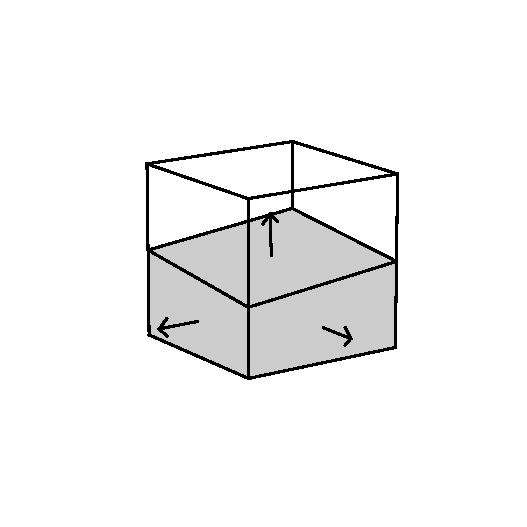
\includegraphics[width=19pc,angle=0]{./figures/cell_diagram}\\
%  \caption{C grid cell with cloud surface.}\label{fig:cell_diagram}
%\end{figure}

\begin{figure}[t]
  \noindent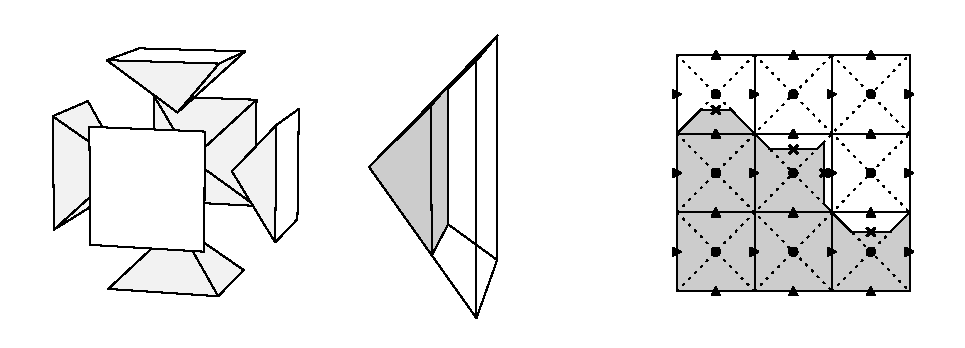
\includegraphics[width=40pc,angle=0]{./figures/pyramid_scheme}\\
  \caption{Schematic representation of the pyramidal interpolation scheme.
Left panel shows the subdivision of the model grid cell into six pyramids.  
Center panel shows the interpolation of the cloud surface within a 
sub-pyramid between points at the  apex and the center of the pyramid base.  
Right panel shows a horizontal slice through the model's Arakawa C-grid.  
Rightward pointing triangles represent u-velocity points, upward pointing 
triangles represent v-velocity points, circles represent bulk tracer 
quantities, and x represents the location of the cloud surface interpolation
points.  Dotted lines show the boundaries of the pyramidal subdivision of the 
grid, and grey shading represents cloud volume.}\label{fig:pyramid_scheme}
\end{figure}

\begin{figure}[t]
  \noindent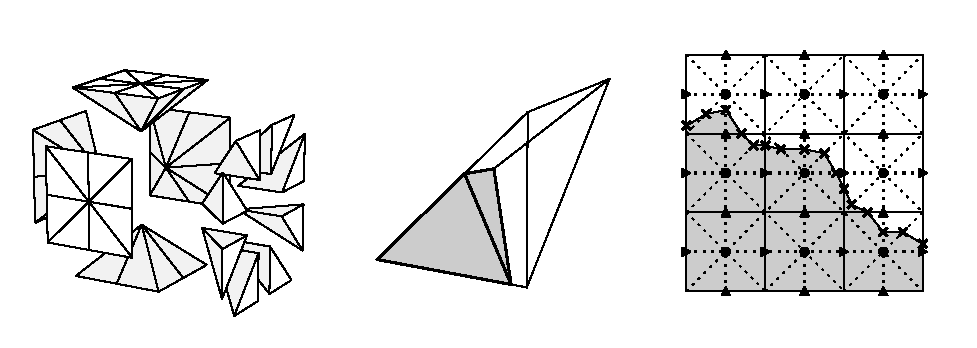
\includegraphics[width=40pc,angle=0]{./figures/tetrahedral_scheme}\\
  \caption{Schematic representation of the tetrahedral interpolation 
scheme.  Left panel shows the subdivision of the model grid cell into forty-
eight tetrahedrons.  Center panel shows the interpolation of the cloud surface
within a sub-tetrahedron between points at the four vertices of the 
tetrahedron.  Right panel shows a horizontal slice through the model's Arakawa 
C-grid.  Rightward pointing triangles represent u-velocity points, upward 
pointing triangles represent v-velocity points, circles represent bulk tracer
quantities, and x represents the location of the cloud surface interpolation
points.  Dotted lines show the boundaries of the tetrahedral subdivision of the 
grid, and grey shading represents cloud volume.}\label{fig:tetrahedral_scheme}
\end{figure}

\begin{figure}[t]
  \noindent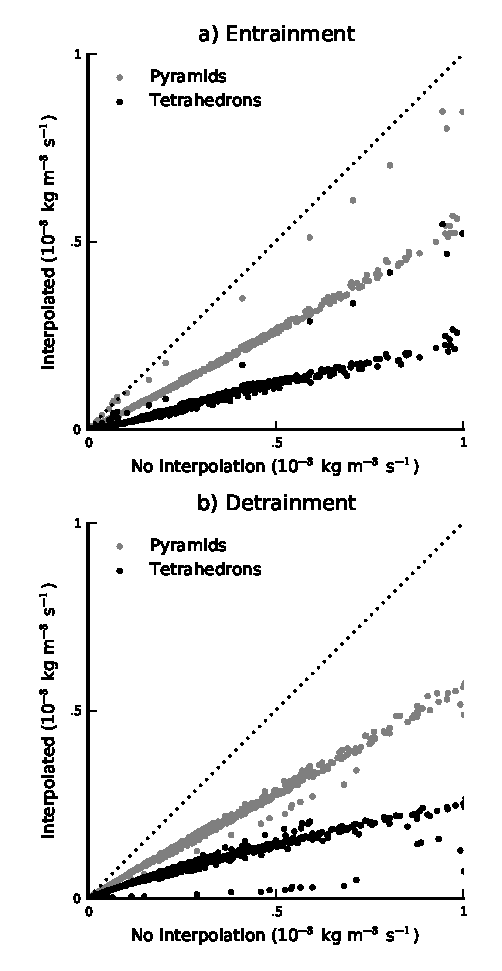
\includegraphics[width=19pc,angle=0]{./figures/effect_of_interpolation}\\
  \caption{Comparison between a) entrainment and b) detrainment values 
calculated directly from fluxes using no surface interpolation vs pyramidal 
surface interpolation (grey) and no surface interpolation vs tetrahedral 
surface interpolation (black).}\label{fig:effect_of_interpolation}
\end{figure}

\begin{figure}[t]
  \noindent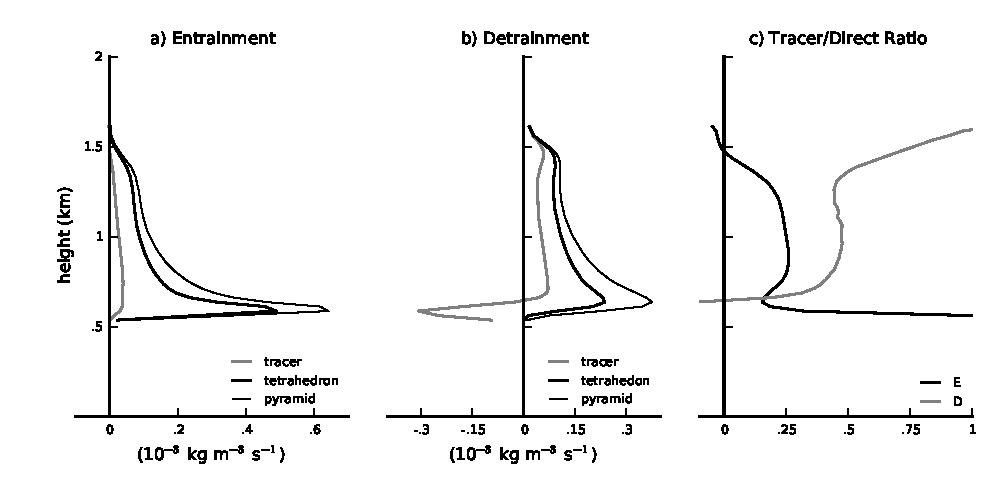
\includegraphics[width=40pc,angle=0]{./figures/direct_vs_tracer_core}\\
  \caption{Comparison of mean model profiles of core a) entrainment and b) 
detrainment calculated using bulk tracer calculations (grey line), direct flux
calculations using pyramidal interpolation (thin black line), and direct flux
calculations using tetrahedral interpolation (thick black line).  c) Ratio of 
bulk tracer rates to direct flux using tetrahedral interpolation rates of
entrainment (black) and detrainment (grey).  d) and e) are the same as 
a) and b) but for the fractional entrainment and detrainment rates.}\label{fig:direct_vs_tracer}
\end{figure}

\begin{figure}[t]
  \noindent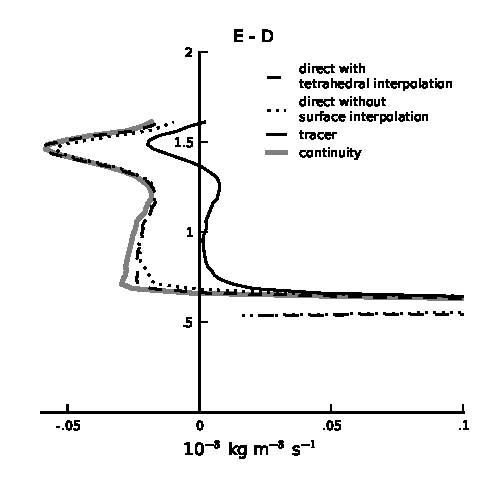
\includegraphics[width=19pc,angle=0]{./figures/E_minus_D_core}\\
  \caption{Average profiles of entrainment minus detrainment calculated using 
direct fluxes with tetrahedral surface interpolation (dashed line), direct 
fluxes with no surface interpolation (dotted line), bulk tracer calculations 
(black line), and the continuity equation (grey line).}\label{fig:E_minus_D}
\end{figure}

\begin{figure}[t]
  \noindent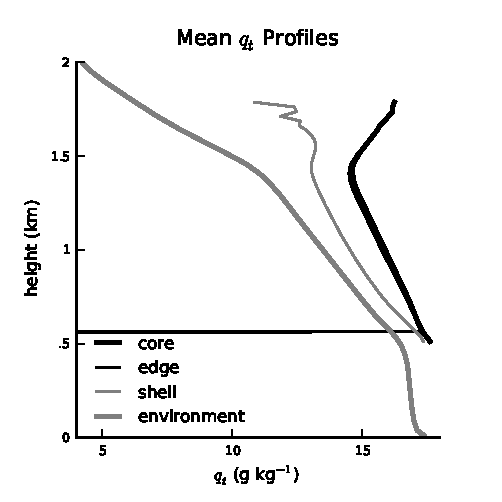
\includegraphics[width=19pc,angle=0]{./figures/shell_edge_profiles_core}\\
  \caption{Mean profiles of $q_t$ in the cloud core (thick grey line), core 
edge (thin black line), core shell (thin grey line), and environment (thick 
black line).}\label{fig:shell_edge_profiles}
\end{figure}

\begin{figure}[t]
  \noindent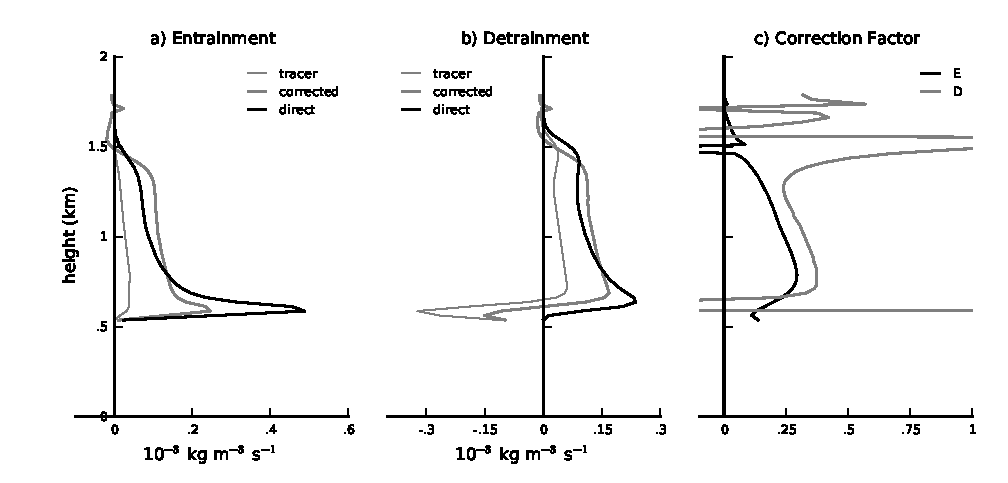
\includegraphics[width=40pc,angle=0]{./figures/corrected_entrainment_core}\\
  \caption{Comparison of mean a) entrainment and b) detrainment profiles 
calculated using uncorrected bulk tracer budgets (thin grey line), bulk tracer 
budgets corrected for the presence of a moist cloud shell (thick grey line), and
direct flux calculations with tetrahedral surface interpolation (black line).
c) Ratio of corrected bulk tracer rates to the direct flux using
tetrahedral interpolation rates of entrainment (black) and detrainment (grey).
d) and e) are the same as a) and b) but for the fractional entrainment and
detrainment rates.}\label{fig:corrected_entrainment}
\end{figure}

\begin{figure}[t]
  \noindent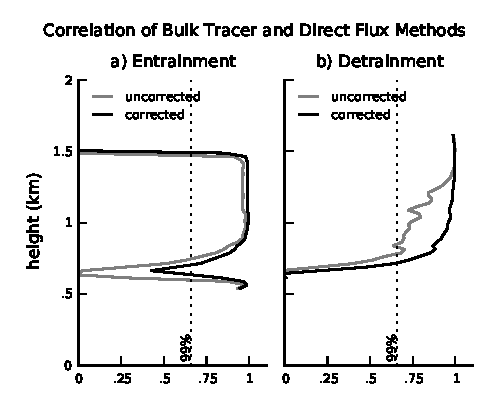
\includegraphics[width=19pc,angle=0]{./figures/correlations_core}\\
  \caption{Profiles of the correlation between direct entrainment calculations
with tetrahedral surface interpolation and either uncorrected (grey lines) or 
corrected (black lines) bulk tracer calculations for a) entrainment and b) 
detrainment.  Dotted line shows the 99\% confidence level for a significant 
correlation.}\label{fig:correlations}
\end{figure}

\begin{figure}[t]
  \noindent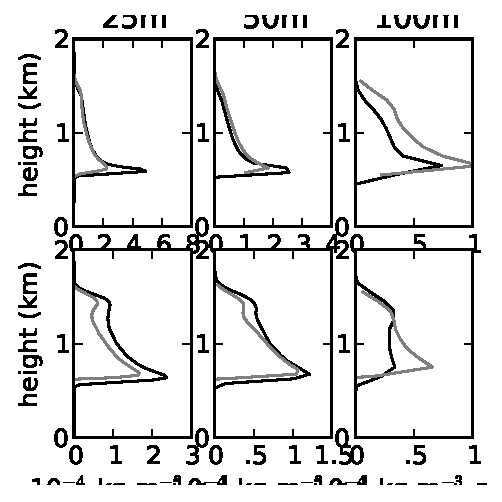
\includegraphics[width=40pc,angle=0]{./figures/resolution_dependence_core}\\
  \caption{Mean entrainment (top row) and detrainment (bottom row) calculated
at 25m (left column), 50m (center column), and 100m (right column) grid 
spacing using direct flux calculations with tetrahedral surface interpolation 
(black line), bulk tracer calculations (thick grey line) and bulk tracer 
calculations corrected for the presence of the moist cloud shell (thin grey 
line).}\label{fig:resolution_dependence}
\end{figure}

\end{document}
